\documentclass[a4paper,12pt]{article}
\usepackage{outline}
\usepackage{pmgraph}
\usepackage[normalem]{ulem}
\usepackage{comment} % enables the use of multi-line comments (\ifx \fi)
\usepackage{lipsum} %This package just generates Lorem Ipsum filler text.
\usepackage{fullpage} % changes the margin
\usepackage{listings}
\usepackage{color}
\usepackage{mdframed}
\usepackage{listings}
\usepackage{amssymb}
\usepackage{amsmath}
\usepackage{graphicx}
\graphicspath{ {../screenshots/} }
\renewcommand{\lstlistingname}{Code Block}% Listing -> Algorithm
\renewcommand{\lstlistlistingname}{List of \lstlistingname s}% List of Listings -> List of Algorithms

\linespread{1.5}
%--------------------Indention
\setlength{\parindent}{15pt}
\lstset{frame=shadowbox, rulesepcolor=\color{white}}
\mdfsetup{frametitlealignment=\center}
\lstset{
  numbers=left,
  stepnumber=1,
  firstnumber=1,
  numberfirstline=true
}

\begin{document}
\section*{Objective}

\hspace{15pt}In this lab, a fast-adder circuit for two-opperand addition was designed called carry-lookahead addition. The design consists of using a combination of dataflow and structural Verilog. The designs were then simulated on the Xilinx ISE to check for correctness. The propagation delays for for a 4-bit and 16-bit carry-lookahead adder were also analyzed in order to compare to similar sized ripple-carry adders.  

\section*{Design}

% EXP 1
% generate propagate unit
% carry lookahead unit
% summation unit
% carry lookahead 4bit
% 4-bit carry lookahead adder
% modified to 2ns gate delays - propagation was measuered
% \lstinputlisting[language=Verilog,,caption=4-Bit ALU ]{../code/code name.v}
% EXP 2
% block_carry_lookahead_unit.v
% \lstinputlisting[language=Verilog,,caption=4-Bit ALU ]{../code/block_carry_lookahead_unit.v}
% GPU and SU changed to be 16 bit wide with removed gate delay
% \lstinputlisting[language=Verilog,,caption=4-Bit ALU ]{../code/code name.v}
% top level module carry_lookahead_16bit
% \lstinputlisting[language=Verilog,,caption=4-Bit ALU ]{../code/code name.v}
% Edit test bennch TEST_DELAY (9ns)
% \lstinputlisting[language=Verilog,,caption=4-Bit ALU ]{../code/code name.v}

\textbf{Experiment 1}

To start off the experiment, the following code was written for the most part as part of the prelab. A few modifications were made into order to function properly. The first three blocks of code are of the modules (\textit{generate-propagate-unit, carry-lookahead-unit,} and \textit{summation-unit}) used in \textit{Code Block 4} for the top level   module \textit{carry-lookahead-4bit}

% Verilog code template
  \lstinputlisting[language=Verilog,,caption=Generate Propagate Unit (4-Bit)]{../code/generate_propagate_unit.v}

  \lstinputlisting[language=Verilog,,caption=Carry Lookahead Unit (4-Bit)]{../code/carry_lookahead_unit.v}
  
  \lstinputlisting[language=Verilog,,caption=Summation Unit (4-Bit)]{../code/summation_unit.v}
  
  \lstinputlisting[language=Verilog,,caption=Top Level Carry Lookahead (4-Bit)]{../code/carry_lookahead_4bit.v}
  
  For the next part, gate delays were modified in the following modules.
  
  \lstinputlisting[language=Verilog,firstnumber=8,firstline=8,lastline=9,caption=Generate Propagate Unit (4-Bit with Delay)]{../code/generate_propagate_unit_delay.v}

  \lstinputlisting[language=Verilog,firstnumber=8,firstline=8,lastline=14,caption=Carry Lookahead Unit (4-Bit with Delay)]{../code/carry_lookahead_unit_delay.v}
  
  \lstinputlisting[language=Verilog,firstnumber=8,firstline=8,lastline=8,caption=Summation Unit (4-Bit with Delay)]{../code/summation_unit_delay.v}

  \hspace{-15pt}\textbf{Experiment 2}
  
  In the next experiment, a block carry lookahead unit was designed. The module interface is as follows:

  \lstinputlisting[language=Verilog,,caption=Block Carry Lookahead Unit]{../code/block_carry_lookahead_unit.v}
  
  Next, the generate propegate unit and summation unit were modified in order to take in 15 bit wires as shown below. The gate delays were also removed.
  
  \lstinputlisting[language=Verilog,firstnumber=4,firstline=4,lastline=5,caption=Generate Propagate Unit (16-Bit)]{../code/generate_propagate_unit_delay.v}
  
  \lstinputlisting[language=Verilog,firstnumber=4,firstline=4,lastline=5,caption=Summation Unit (16-Bit)]{../code/summation_unit_delay.v}
  
  Finally the past modules were implemented into a top−level module for a 16-bit carry lookahead adder.
  
  \lstinputlisting[language=Verilog,,caption=16-Bit Carry Lookahead Adder]{../code/carry_lookahead_16bit.v}
  
\newpage

\section*{Results}

  \textbf{Experiment 1}
  
  Below is the waveform for the 4-Bit carry lookahead adder.

\begin{figure}[h]
  \begin{center}
    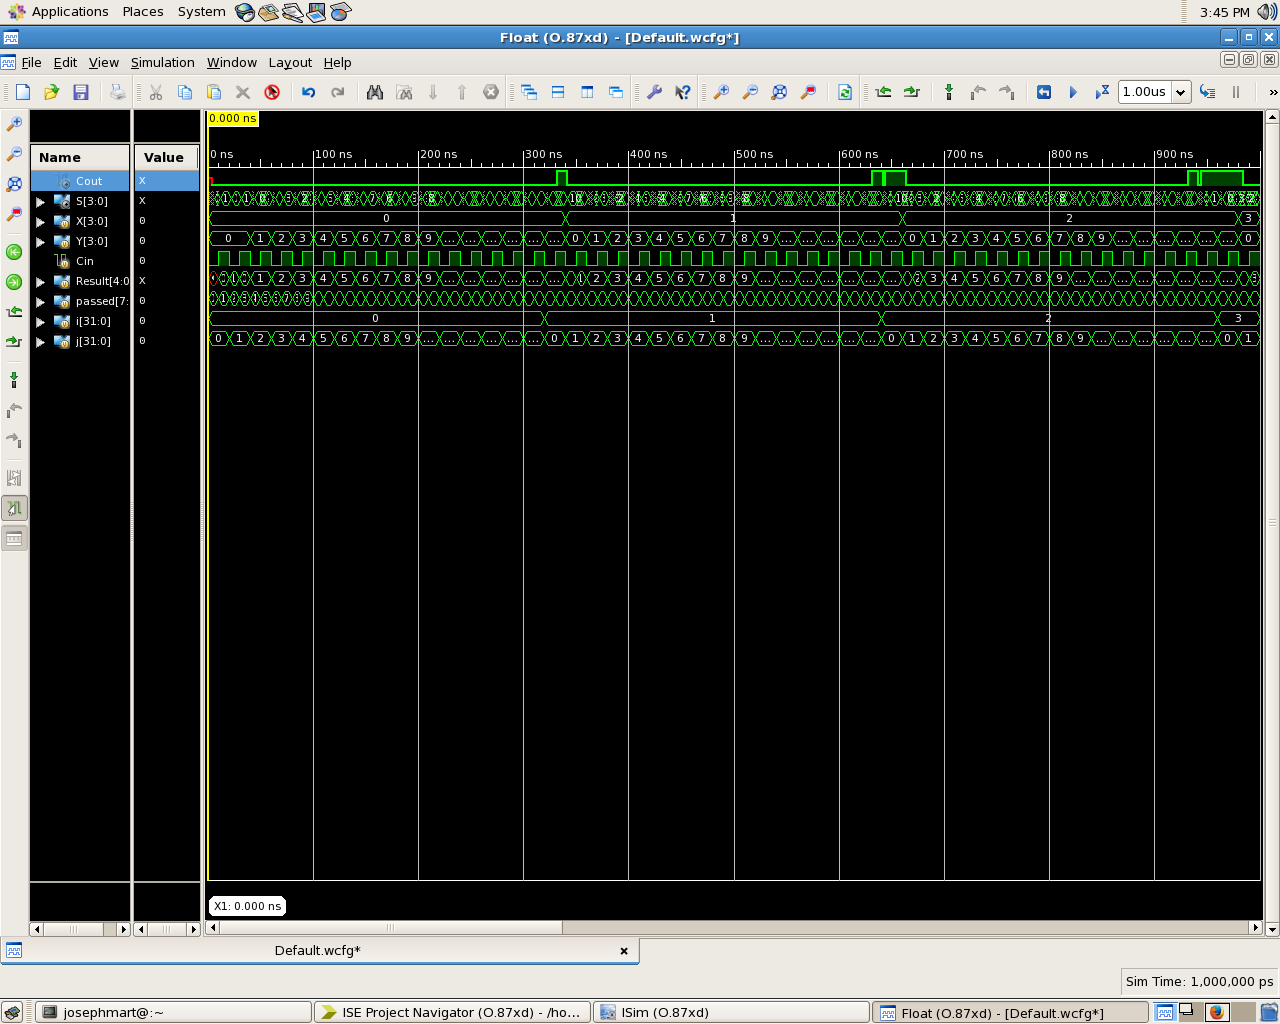
\includegraphics[scale=.2]{exp1_full_waveform.png}
    \caption{\textit{Full waveform}}
  \end{center}
\end{figure}

Below are the test results for the same module where all the tests results passed.

\begin{figure}[h]
  \begin{center}
    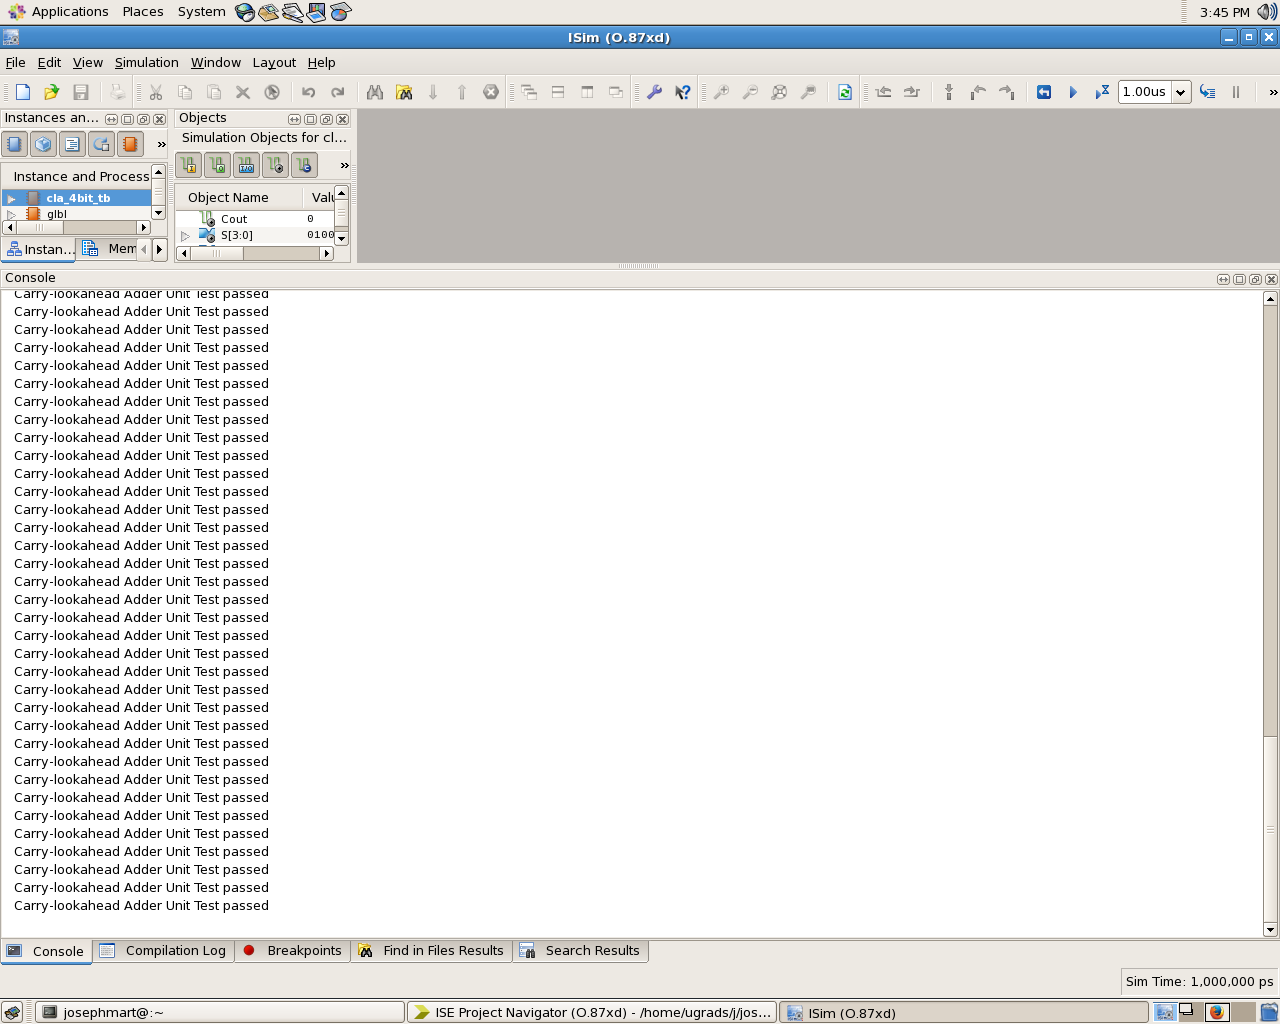
\includegraphics[scale=.15]{exp1_test_results.png}
    \caption{\textit{Experiment 1 Test Results}}
  \end{center}
\end{figure}

\newpage
  Below is the waveform with the gate delays added.
  
\begin{figure}[h]
  \begin{center}
    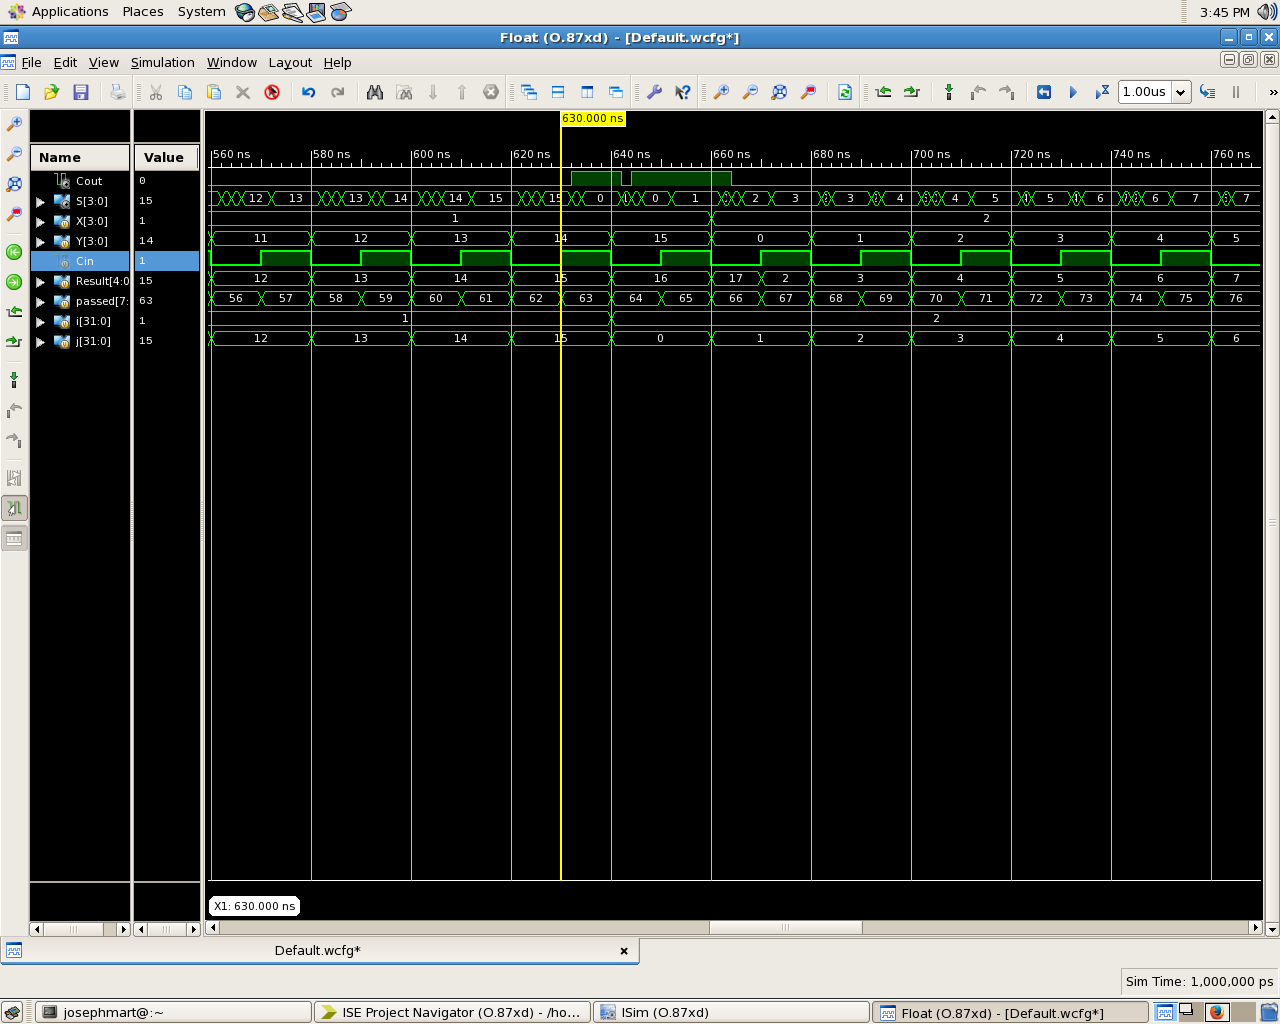
\includegraphics[scale=.2]{Exp_1_difference_6ns.png}
    \caption{\textit{Difference 6ns}}
  \end{center}
\end{figure}

\textbf{Experiment 2}

  Below is the first time the tests failed for 16 bit carry lookahead adder. The TEST\_DELAY was set to $9$ ns

\begin{figure}[h]
  \begin{center}
    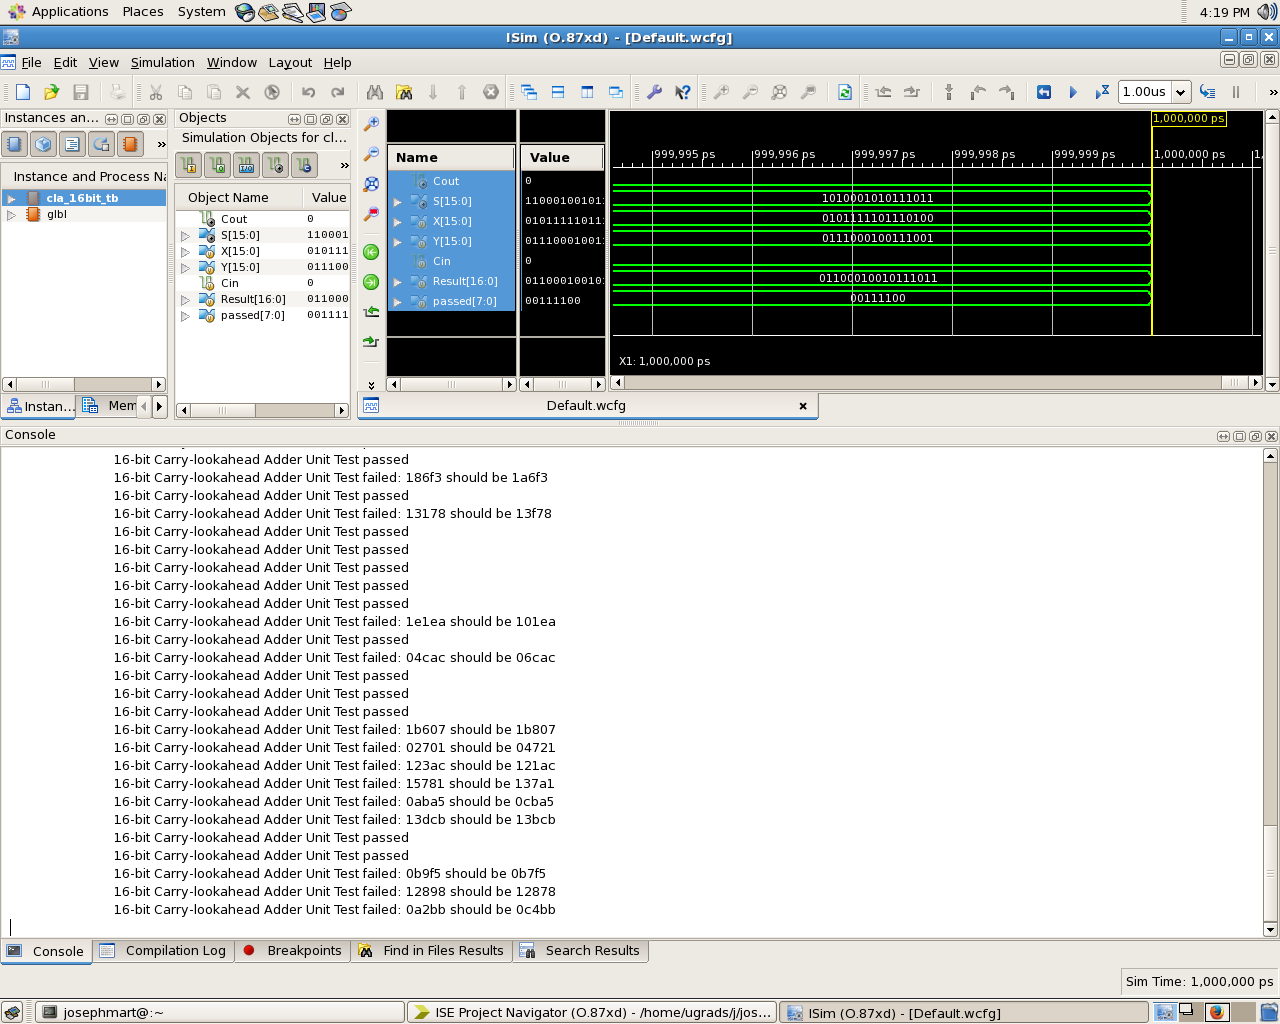
\includegraphics[scale=.15]{exp3_failed_tests.png}
    \caption{\textit{Experiment 3 Failed Tests}}
  \end{center}
\end{figure}

\newpage

\begin{figure}[h]
  \begin{center}
    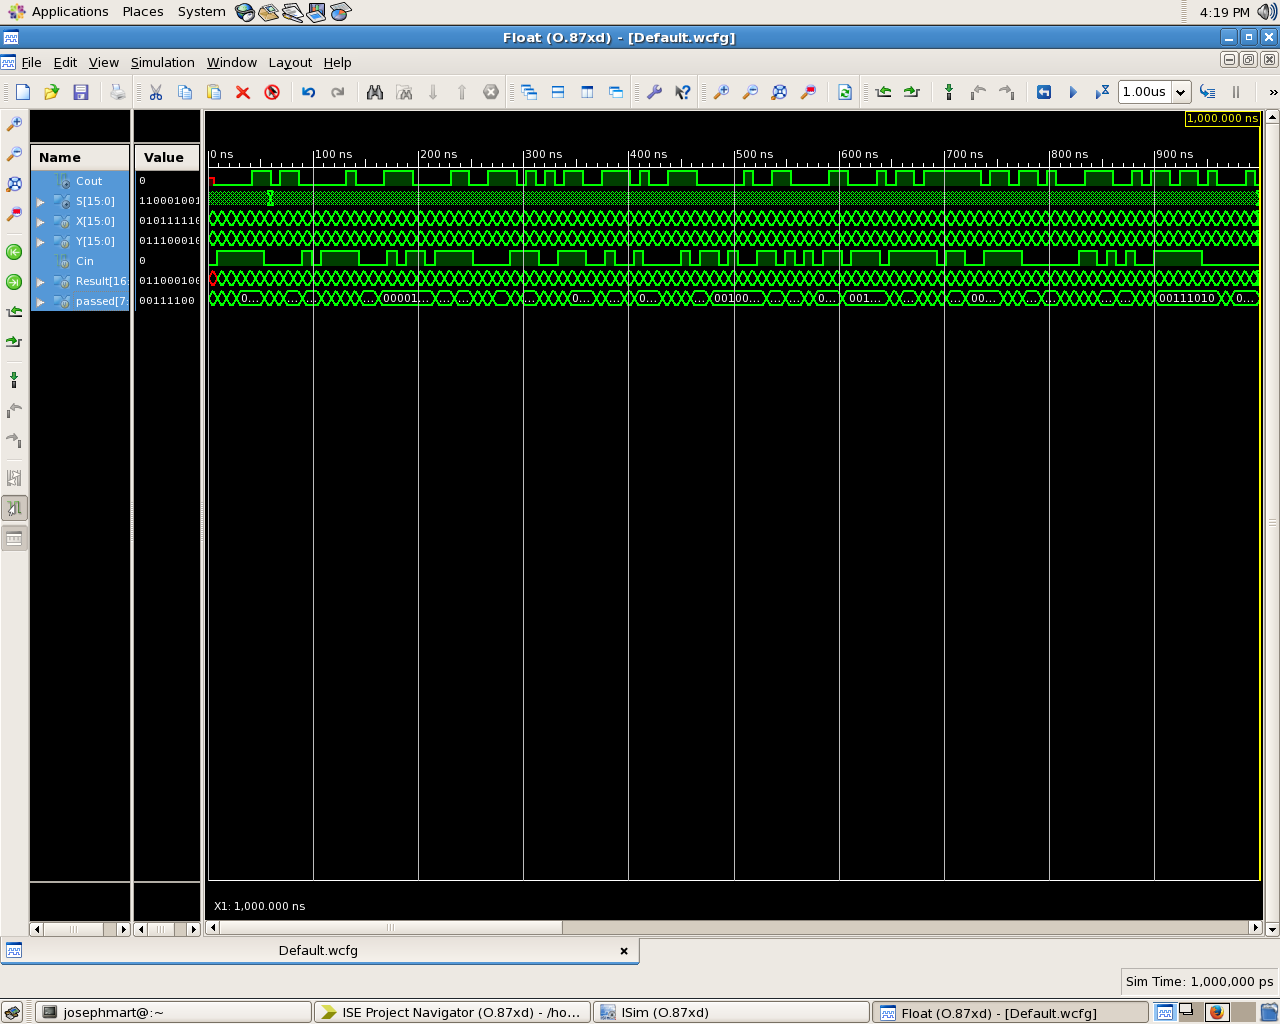
\includegraphics[scale=.2]{exp3_failedWaveform.png}
    \caption{\textit{Failed Waveform}}
  \end{center}
\end{figure}


\section*{Conclusion}

  In conclusion, I learned how faster adders than ones previously created are designed. This lab also allowed me to build upon my ability to create basic modules using both structural and dataflow Verilog. After creating a 4-Bit adder, I was able to create a 16-bit lookahead adder using and modifying previously created modules.

\section*{Questions}

\begin{enumerate}
  \item \textbf{Include the source code with comments for all modules in lab. you do not have to include test bench code. Code without comments will not be accepted!}
    \textit{In report}
  \item \textbf{Include the simulation screenshots requested in the above experiments in addition to the corresponding test bench console output.}
      \textit{In report}
  \item \textbf{Answer all questions through the lab manual: If your calculations in the prelab are correct and you correctly added delays to your sub-modules,
you should find that the computed delay matches the measure delay. Is this the case?}
  No they do not match. I believe the issue is with how gate delays were not assigned correctly.
  
  \item \textbf{How does the gate-count of the 16-bit carry-looahead adder compare to that of a ripple-carry adder of the same size.}
  
  The gate-count of a 16-bit-carry-lookahead adder compared to a ripple-carry of the same size is that CLA has 82-gates and RC has 80 gates. Also the CLA functions faster than the RC.
  
  \item \textbf{How does the propagation delay of the 4-bit carry-lookahead adder compare to that of a ripple-carry adder of the same size. Similarly, how does the 16-bit carry-lookahead adder compare to that of a ripple-carry adder of the same size.}
  
  The propagation delay of a 16-bit carry lookahead adder compared to a ripple carry adder is that the 16-bit CLA has a bigger delay than the RC. This is due to how the CLA uses parallel circuitry rather than a long string of full adders in series like the RC.
  
\end{enumerate}

\section*{Student Feedback}

\begin{enumerate}
  \item \textbf{What did you like most about the lab assignment and why? What did you like least about it and why?}
  I liked building upon my knowledge of verilog.

  \item \textbf{Were there any section of the lab manual that were unclear? If so, what was unclear? Do you have any suggestions for improving the clarity?}
  The lab was pretty clear

  \item \textbf{What suggestions do you have to improve the overall lab assignment?}
  This was the easiest lab so far so I do not have any suggestions.

\end{enumerate}

\ifx
\begin{thebibliography}{1}
\bibitem{Verilog} Charles Kime \& Thomas Kaminski  \emph{Logic and Computer Design Fundamentals} \\ \hspace{15pt}\textit{http://www.cs.bilkent.edu.tr/~will/courses/CS223/Verilog/LCDF3_Verilog_Ch_4.pdf}
\end{thebibliography}

\section*{Attachments}
%Make sure to change these
Lab Notes, HelloWorld.ic, FooBar.ic
%\fi %comment me out

\begin{thebibliography}{9}
\bibitem{Verilog} Charles Kime & Thomas Kaminski  \emph{Logic and Computer Design Fundamentals} \textit{http://www.cs.bilkent.edu.tr/~will/courses/CS223/Verilog/LCDF3_Verilog_Ch_4.pdf}
\end{thebibliography}

%How to cite
Put your Problem statement here! Example of a Citation\cite[p.219]{Robotics}. Here's Another Citation\cite{Flueck}
\fi
\end{document}
